\documentclass[11pt,a4paper]{article}
\usepackage[margin=2.2cm]{geometry}
\usepackage[T1]{fontenc}
\usepackage{lmodern}
\usepackage{graphicx}
\usepackage{booktabs}
\usepackage{tabularx}
\usepackage{amsmath}
\usepackage{enumitem}
\usepackage{xcolor}
\usepackage[colorlinks=true,linkcolor=blue!50!black,citecolor=blue!50!black,urlcolor=blue!50!black]{hyperref}
\usepackage[numbers,sort&compress]{natbib}
\setlist{itemsep=2pt,topsep=4pt}
\newcolumntype{L}{>{\raggedright\arraybackslash}X}

\title{Timing in VitalDB: a user guide\\[4pt]\large How to judge whether two signals are aligned well enough for your question}
\author{}
\date{Draft, October 2026}

\begin{document}
\maketitle

\begin{abstract}
Every time in a clinical database carries two kinds of uncertainty: how far it may be from the true time
(\emph{accuracy}) and how wide an interval it stands for (\emph{resolution}). In VitalDB these range from about a
millisecond for waveform samples to five minutes for anaesthesia records and a whole day for admission dates. This
guide summarises what we measured for each kind of time, gives a rule of thumb for deciding whether two signals can
be compared at the timescale of a research question, and works through examples. It follows the framework of
Goodwin et al.~\cite{goodwin2022timing} and applies it to VitalDB~\cite{lee2022vitaldb}.
\end{abstract}

\noindent\fbox{\parbox{\linewidth}{\small\textbf{Note (October 2026).} This guide uses the \emph{accuracy} and
\emph{resolution} of Goodwin et al.~\cite{goodwin2022timing}. The metrology atlas (vitaldb.metrology-atlas.org) now
states the same quantities in the vocabulary of the VIM and GUM: a systematic error (bias), corrected where known, and
a standard uncertainty with named components, the interval a value describes being part of what the value is. Its
numbers supersede the ones here; in particular the raw BIS stamps come about 0.79\,s \emph{early}, not late.}}

\section{Why timing matters}
Most analyses of VitalDB compare things recorded by different devices or people: a drug infusion and a blood
pressure response, a laboratory result and the waveforms around it, an anaesthesia event and a monitor trend. Each
source has its own clock, its own delay and its own rounding. Goodwin et al.~\cite{goodwin2022timing} describe how
such timing errors arise in clinical databases and why they are easy to overlook: the data look precise, because
every value carries a timestamp to the millisecond, even when the event it describes is known only to the nearest
few minutes. This guide makes those uncertainties explicit for VitalDB, so you can check before you analyse.

\section{Two numbers for every time}
\begin{description}
\item[Accuracy] The offset between a recorded time and the true time on a common reference. Here the reference is
the recorder clock, as reconstructed from the SNUADC sample count (the \emph{stamp model}). Accuracy includes clock
offsets, transmission and processing delays, and documentation lag.
\item[Resolution] The width of the interval a time stands for. A 500\,Hz sample stands for 2\,ms. A heart rate
averaged over 6\,s stands for 6\,s, even though its stamp is to the millisecond. An event entered on a five-minute
grid stands for five minutes.
\end{description}
Two further points matter in practice:
\begin{itemize}
\item \textbf{The stamp is not the event.} A numeric value is stamped when the monitor reports it, which is after
its averaging window closes. Treat the stamp as the time the value became \emph{available}, not the time the
physiology happened. This is also the rule to follow to avoid leaking future information into a prediction model.
\item \textbf{Rounding direction matters.} If a time is rounded up, the true time lies before it; if rounded to
nearest, it lies on either side. Section~\ref{sec:emr} shows that VitalDB's five-minute anaesthesia entries are
rounded up.
\end{itemize}

\section{The accuracy and resolution map}
Figure~\ref{fig:map} places every kind of time in VitalDB on one log--log map. Each ellipse spans the measured (solid)
or estimated (dashed) range on each axis. Arrows run from raw device stamps to their position after
synchronisation. The key gives the evidence for each ellipse.

\begin{figure}[htbp]
\centering
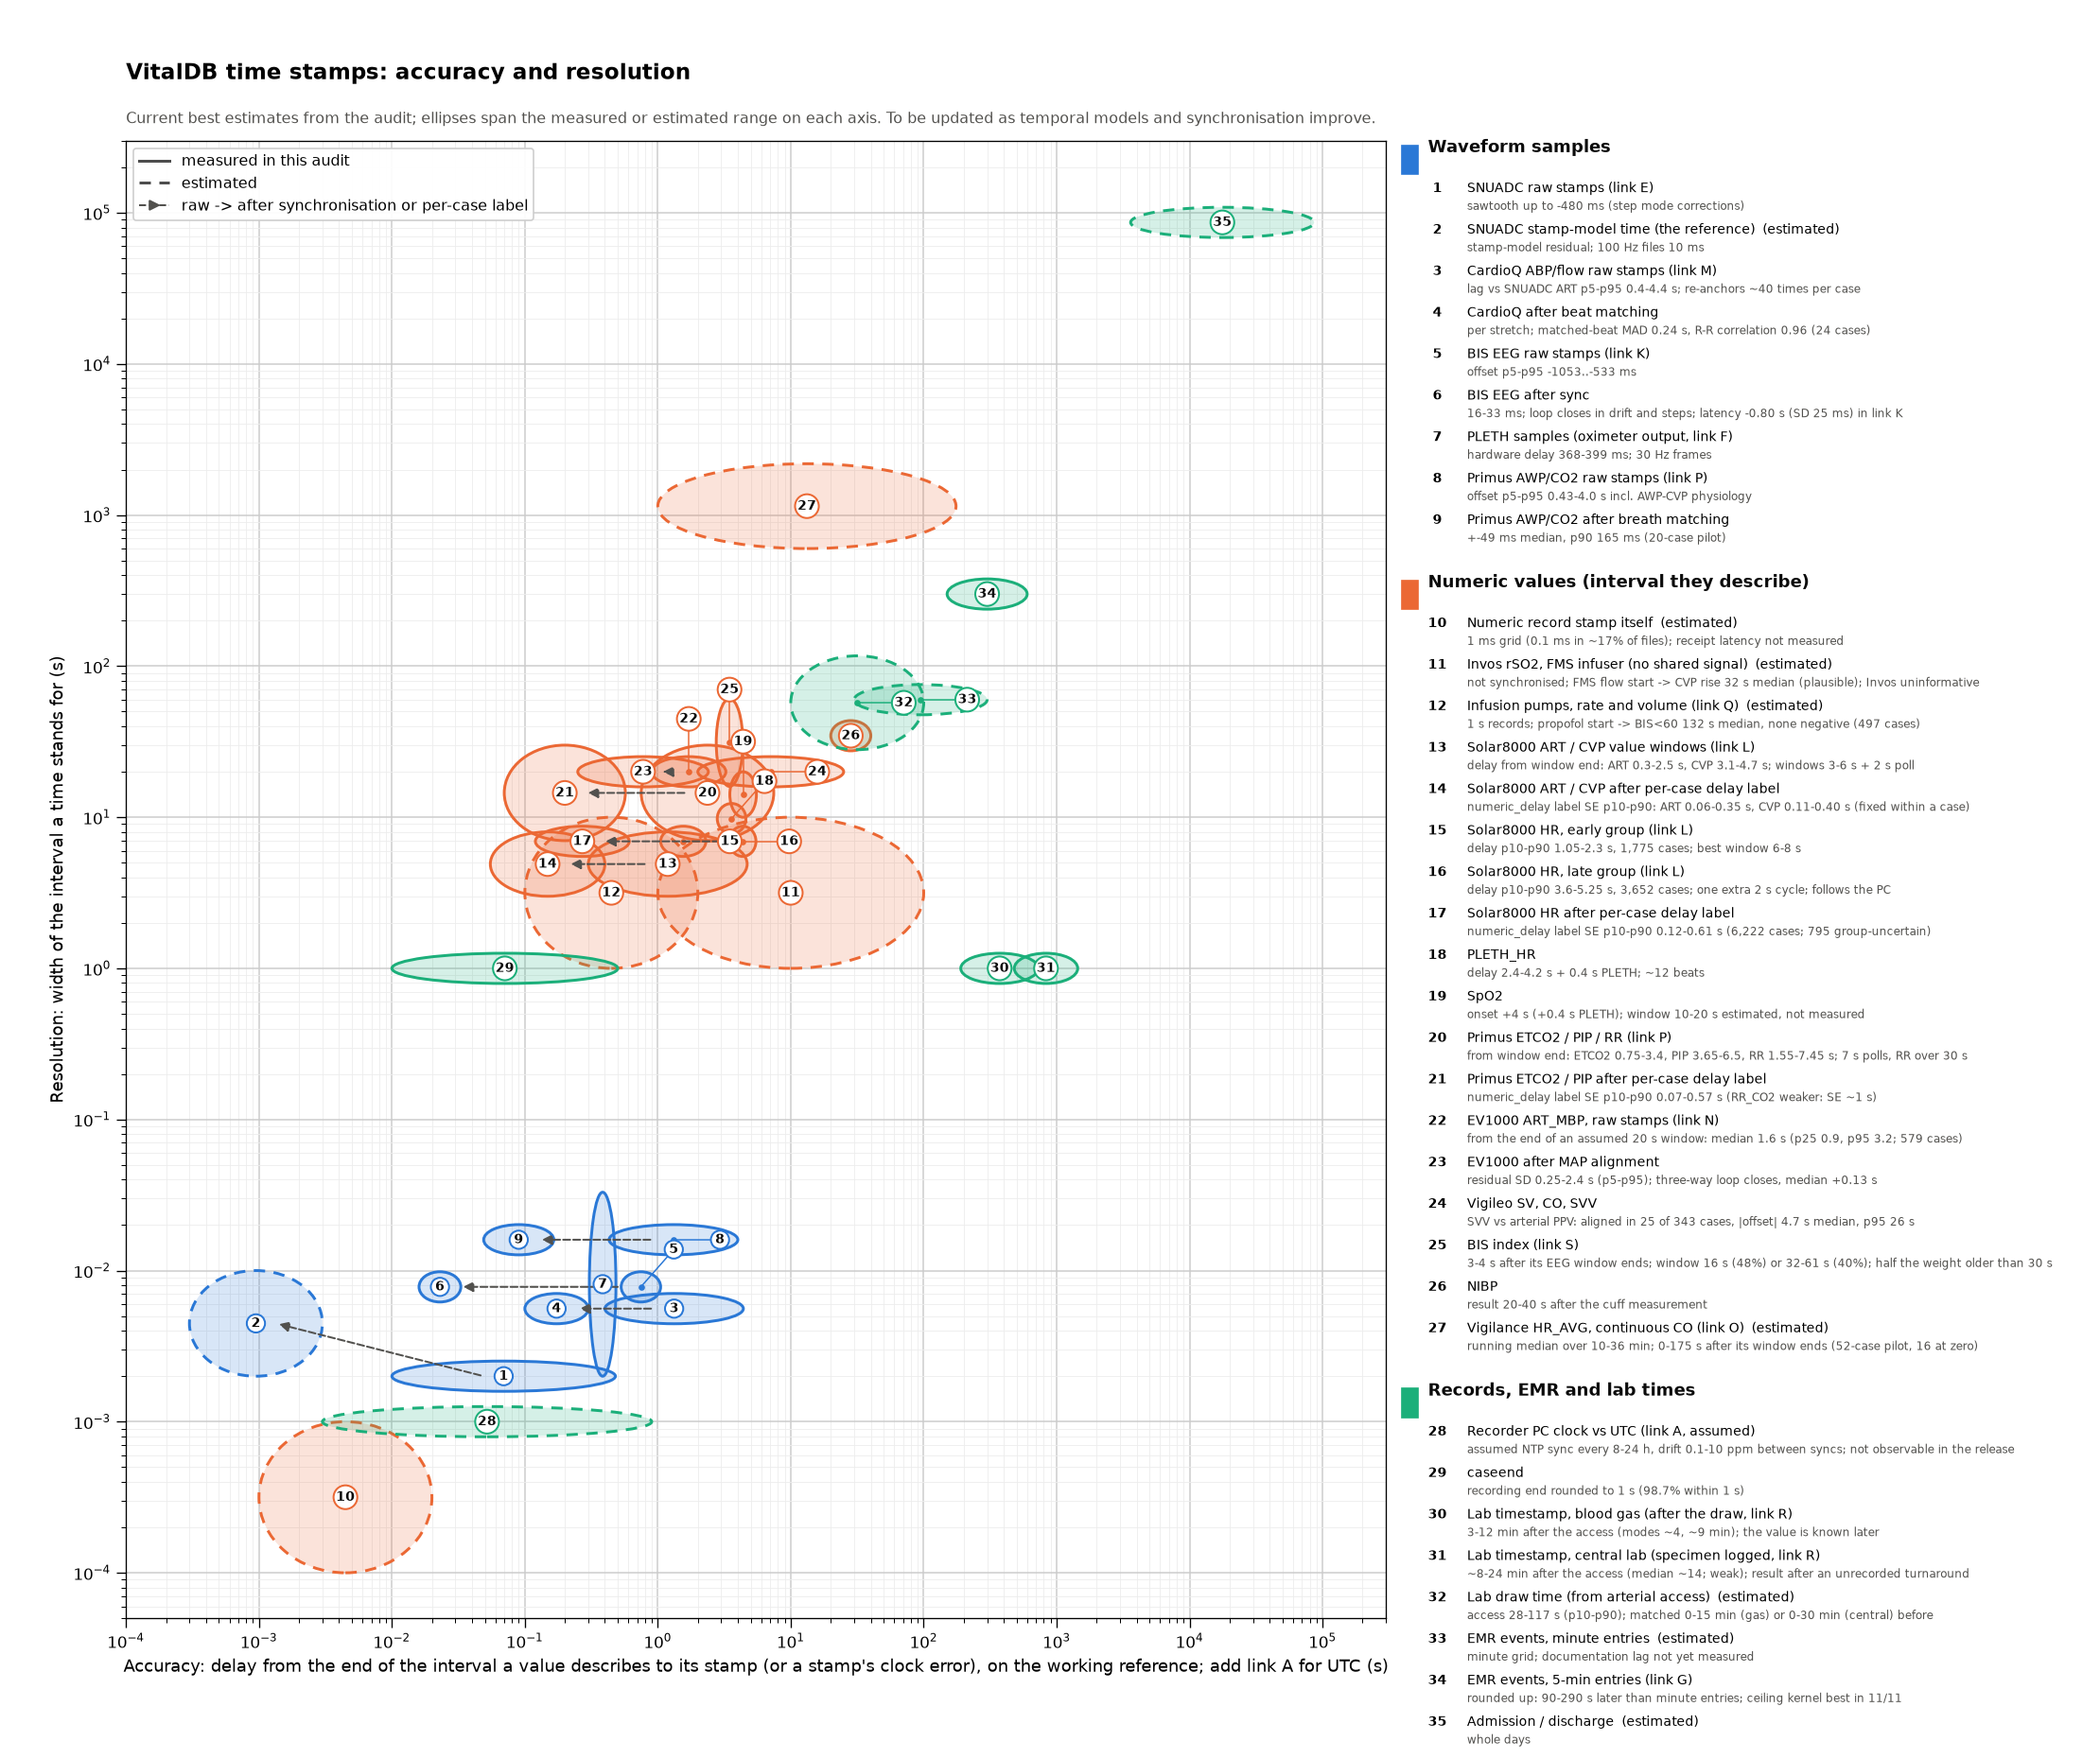
\includegraphics[width=\textwidth]{time_source_accuracy.png}
\caption{Accuracy (offset from the recorder clock, $x$) and resolution (width of the interval a time stands for,
$y$) for each kind of time in VitalDB. Blue: waveform samples. Orange: numeric values. Green: records, anaesthesia
(EMR) and laboratory times.}
\label{fig:map}
\end{figure}

Table~\ref{tab:summary} lists typical values. Numbers are medians or ranges over the cases examined; your case may
differ.

\begin{table}[htbp]
\centering
\small
\begin{tabularx}{\textwidth}{@{}l L L@{}}
\toprule
Source & Accuracy (offset) & Resolution \\
\midrule
SNUADC waveforms (ECG, ART, PLETH, CVP) & reference; raw stamps sawtooth up to $\sim$480\,ms & 2--10\,ms (100--500\,Hz) \\
BIS EEG & $-1.05$ to $-0.53$\,s raw; 16--33\,ms after sync & 7.8\,ms (128\,Hz) \\
Primus airway pressure and CO$_2$ & 0.4--4\,s raw; $\sim$50\,ms after breath matching & 16\,ms (62.5\,Hz) \\
CardioQ ABP and flow & 0.4--4.4\,s raw; $\sim$0.24\,s after beat matching & 5.6\,ms (180\,Hz) \\
Solar8000 HR, ART, CVP & 1.9--5\,s after the averaging window closes & 3--6\,s windows plus 2\,s polling \\
SpO$_2$ and PLETH\_HR & onset $\sim$4\,s & 10--20\,s smoothing ($\sim$12 beats for PLETH\_HR) \\
Primus ETCO$_2$, PIP, RR & 1.8--8.5\,s & last breath to 30\,s; $\sim$7\,s records \\
EV1000 ART\_MBP & 1.6\,s median, p95 3.3\,s & 20\,s \\
Vigilance HR\_AVG & window centre 6--21\,min behind & running median over $\sim$20--30\,min \\
NIBP & result 20--40\,s after the cuff measurement & one reading \\
Infusion pumps (Orchestra) & $\sim$1\,s; propofol $\rightarrow$ BIS response 132\,s median & 1\,s records \\
Anaesthesia/operation events, 5-min entries & rounded up: true time 0--300\,s earlier & 300\,s \\
Anaesthesia events, minute entries & documentation lag (minutes) & 60\,s \\
Laboratory results & result 3--12\,min after the sample & draw time not recorded \\
Admission, discharge & --- & 1 day \\
\bottomrule
\end{tabularx}
\caption{Typical accuracy and resolution by source.}
\label{tab:summary}
\end{table}

\section{Rule of thumb}\label{sec:rule}
To decide whether two signals A and B can be compared for a given question:
\begin{enumerate}
\item \textbf{Find both on the map}, at their synchronised position if you apply the synchronisation.
\item \textbf{Take the largest edge.} For each ellipse, read its right edge (worst accuracy) and its top edge
(widest resolution). The relative alignment uncertainty $U$ is the largest of these four numbers:
\[
U \approx \max\left(a_A,\; a_B,\; r_A,\; r_B\right).
\]
If A and B come from the same device clock (for example ECG and ART, both from SNUADC), their offsets cancel:
drop $a_A$ and $a_B$ and use the resolutions alone. Prefer the right edge to the centre, so the estimate is
conservative.
\item \textbf{Compare with the timescale $T$ of your question}, the shortest time difference your conclusion depends
on:
\begin{itemize}
\item $U < T/10$: \textbf{safe}. Timing error will not change your answer.
\item $T/10 \le U \le 10\,T$: \textbf{marginal}. Model the uncertainty explicitly (for example, treat times as
uniform intervals, shift by the known lag, or run a sensitivity analysis over the plausible offsets).
\item $U > 10\,T$: \textbf{unsafe}. The data cannot answer the question at this timescale. Ask a coarser
question or use a better-timed source.
\end{itemize}
\end{enumerate}
The rule uses the maximum rather than a sum of squares because the largest term usually dominates by an order of
magnitude, and because offsets are often systematic rather than random.

\section{Worked examples}
\paragraph{1. Pulse arrival time from ECG and arterial waveform.}
Both from SNUADC, same clock: drop accuracy. Resolution 2\,ms each, so $U\approx 2$\,ms (plus up to 0.8\,ms skew
from sequential channel reads). Pulse arrival time is $\sim$200--300\,ms and changes of interest are $\sim$10\,ms:
$U/T \approx 0.2$. \emph{Marginal}: average over beats or interpolate fiducial points.

\paragraph{2. Arterial waveform against the BIS EEG.}
After synchronisation BIS sits at $\sim$33\,ms accuracy; resolution 8\,ms. $U\approx 33$\,ms. For a question about
EEG changes over seconds ($T=1$\,s), $U/T=0.03$: \emph{safe}. Without synchronisation the raw offset is up to
1\,s: \emph{marginal}.

\paragraph{3. Heart rate numeric against arterial pressure numeric.}
Both Solar8000 numerics: same clock, but each value is an average over a window and reported after a delay. The
widest resolution is $\sim$6\,s; delays differ between tracks by $\sim$2\,s. $U\approx 6$\,s. For trends over
minutes, \emph{safe}; for beat-to-beat coupling, use the waveforms instead.

\paragraph{4. Propofol infusion start against BIS.}
Pump records are $\sim$1\,s; BIS is a 1\,s numeric with vendor smoothing (estimated tens of seconds). $U$ is tens of
seconds. The median response is 132\,s, so for onset latency $U/T\approx 0.2$: \emph{marginal}, and the
measured latencies (none negative across 497 cases) are plausible.

\paragraph{5. SpO$_2$ against a drug recorded in the anaesthesia record.}
The anaesthesia entry has 300\,s resolution. For a 30\,s desaturation response, $U/T = 10$: \emph{unsafe}. For
whether saturation fell in the 30 minutes after induction, $U/T = 0.17$: \emph{marginal but usable}.

\paragraph{6. A laboratory value against the waveforms at the time of sampling.}
The result time is 3--12\,min after the draw, and the draw time is not recorded. Using the result time as the sample
time gives $U \approx 12$\,min. Questions on a scale of an hour are marginal; minute-scale questions are unsafe
unless the draw is located from the arterial line access artefact, which brings $U$ down to the access duration
($\sim$0.5--2\,min).

\section{Anaesthesia record times}\label{sec:emr}
Anaesthesia start and end, and operation start and end, are mostly entered on absolute five-minute clock marks
(92--98\% of cases; 52\% for anaesthesia start, which mixes minute and five-minute entries). We compared these times
with device markers on the recorder clock: infusion start and stop, loss and return of BIS, start and end of
ventilation and of end-tidal CO$_2$, and the end of the recording. Across all 6,388 cases, five-minute entries sit
90--290\,s later relative to these markers than minute entries do. For all eleven markers a rounding-up model fits
better than rounding to nearest or down.

\textbf{Practical reading:} for a five-minute entry at time $t$, the true time lies in $(t-300\,\text{s},\,t]$;
the best estimate is $t-150$\,s with a standard deviation of $300/\sqrt{12}\approx 87$\,s, plus any documentation
lag. Minute entries carry 60\,s resolution and their own lag. Do not treat the two kinds as equally precise.

\section{Numerics: lag without editing timestamps}
Monitor numerics are computed from the waveforms over a window and reported after a delay. We fitted the window and
delay for several tracks (for example, Solar8000 HR is close to a median over $\sim$6\,s, reported
$\sim$3.6\,s after the window closes). Three conventions help:
\begin{itemize}
\item Keep the recorded stamps. They are the availability time, which is correct for real-time and prediction
work.
\item When you need the physiological time, subtract the delay \emph{and} half the window to reach the window centre.
\item Treat the window as the resolution of that value when applying the rule of thumb.
\end{itemize}
The connectors for TimeNet and AtriumDB attach these properties as labels that span each recording or signal run,
rather than altering the data.

\section{Value resolution, briefly}
Timing and value resolution interact when a threshold defines an event. SNUADC waveforms are 10-bit: about 1\,mmHg
per count for arterial pressure and 10\,\textmu V for ECG, with the arterial signal saturating near 400\,mmHg and ECG
often clipping. Laboratory values in the released CSV drop trailing zeros, and haematocrit is recorded to an integer
when drawn with a blood gas and to 0.1 otherwise. Check value labels before using thresholds near these limits.

\section{Checklist before you analyse}
\begin{enumerate}
\item List every source your analysis compares and find each on Figure~\ref{fig:map}.
\item Decide whether you need availability time (prediction) or physiological time (mechanism).
\item Apply the rule of thumb at the shortest timescale your conclusion depends on.
\item If marginal, model the uncertainty; if unsafe, change the question or the source.
\item Report the timing assumptions with your results, following the recommendations in~\cite{goodwin2022timing}.
\end{enumerate}

\bibliographystyle{unsrtnat}
\bibliography{references}

\end{document}
